\chapter{Design}

This section describes the modules which make part of the system and each module's responsibility.
It also introduces concepts used extensively throughout the system.


\section{System Architecture}

Urban Sketcher is composed of a set of modules, most of them implemented as singleton classes
for managing subsets of the functionality. The interaction between system components is illustrated
on Figure \ref{fig:block-diagram}.
Implemented modules are shaded blue, while integrated modules are shaded green.

\begin{figure}[!ht]
		\centering
		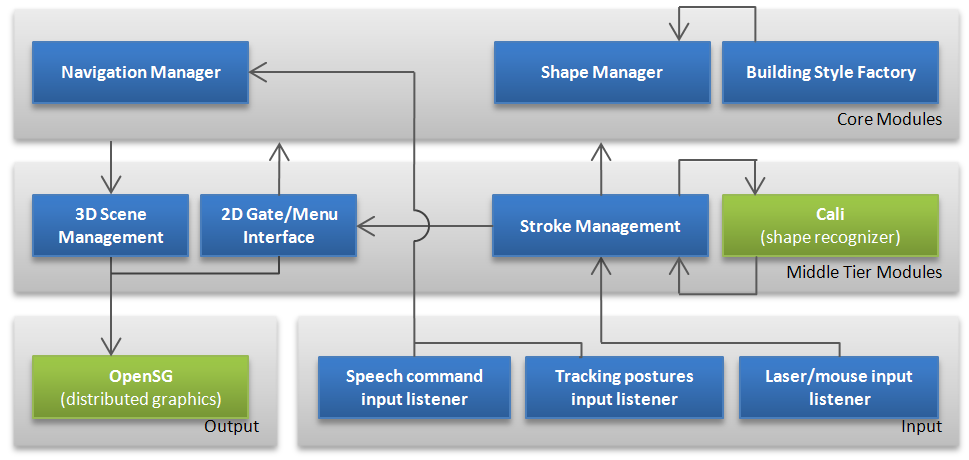
\includegraphics[scale=0.4]{gfx/charts/internal-block-diagram.png}
		\caption{Urban Sketcher Architecture Diagram}
		\label{fig:block-diagram}
\end{figure}

A set of input adapters get data from several media -- laser strokes, mouse pointer events,
speech commands and motion tracked markers' coordinates.
These adapters generate commands which are consumed by higher level managers.

\textbf{Strokes} are managed and at low level, with key stroke gestures triggering commands.
A shape recognition engine named \textbf{Cali} \cite{CALI} was integrated to provide shape detection on 2 cases:
triangle, to invoke the main menu and
rectangle, to identify blueprint sketches over construction planes.
Cali is fed polyline information and returns the recognized shape family and its parameters, if found.
The \textbf{2D Widget Manager} takes care of the visible interface, handling gate and menu events.

The \textbf{Navigation Manager} is responsible for keeping positioning information up to date.
It transforms the positioning state in response to actions issued by the supported navigation modes.

The \textbf{Shape Manager} holds the existing shape references and provides means for them to be selected and manipulated.
It caches loaded shapes to enhance to performance in the generation of buildings, where attached geometry is bound
to repeat.

The \textbf{Building Style Factory} loads and parses style definitions into fa�ade-generating algorithms.
Once fed with blueprint information, desired style and height, this component is able to instantiate
a building and its details.

The \textbf{2D Gate/Menu Interface} is a set of widgets and their logic, affected by strokes.
The widgets make use of the Model-View-Controller \cite{DESPAT} design pattern, with the controller ultimately making use of
higher level managers functionalities.
These widgets are oftentimes created by composition of simpler, general purpose widgets.

Both shapes and 2D widgets know how to render themselves on OpenSG, so they both interact with it.
\textbf{3D Scene Management} handles the representation of the virtual world and is controlled by both the Shape and Navigation
managers.

\section{Urban Sketcher Input/Output Communication}

\begin{figure}[!ht]
		\centering
		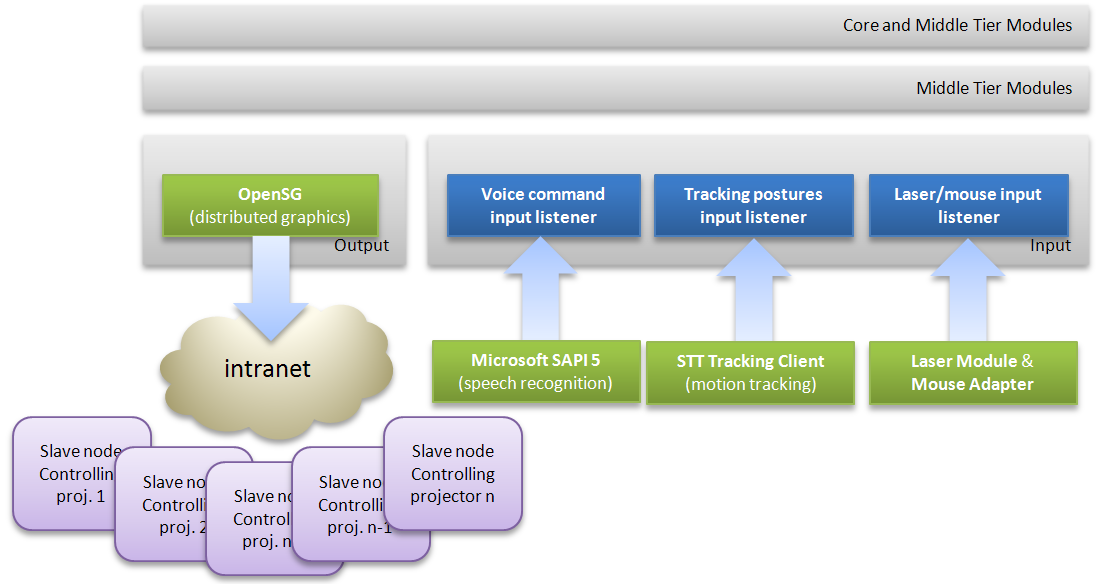
\includegraphics[scale=0.4]{gfx/charts/external-block-diagram.png}
		\caption{Urban Sketcher input/output Diagram}
		\label{fig:ext-block-diagram}
\end{figure}

Urban Sketcher gets input from several media (see Fig.\ref{fig:ext-block-diagram}):
laser pointers, the server machine's mouse and optionally voice commands and tracking postures.
The system renders real-time views to any number of slave machines.
An XML configuration allows parameterizing the range of affected machines and topology of the rendering slaves,
so rendering solely on the server, to a large screen display or both is a matter of switching configurations.

Both the speech command and tracking postures input listeners are fed by simple
application of the available APIs from respectively Microsoft and STT.
The laser input listener receives data from the laser tracking module, work developed by Ricardo Jota \cite{IMMIVIEW-EPCG}.

\section{Stroke-Based Input Interface}

This section details the concepts used for the implementation of the system user interface.

\subsection{Strokes}

A stroke is the result of continuous input from one laser pointer, from the time the laser
light button is pressed until it is released. 
By using the laser detection module, the system gets a stream of laser readings which
come sequentially tagged, that is, the module identifies with reasonable success when different strokes
occur simultaneously, returning both readings tagged with different stroke IDs.
Even so, the module can't infer whether different strokes came from the same source laser pointer.
This limitation sets an important assumption in our system -- one can not know whether 2 strokes came
from the same user, therefore operations must take place during at most the stroke period.
Strokes can also be emulated by using a mouse and pressing the button as if it were a laser pointer.


\subsection{Gates}

The most common activation action in current Graphical User Interface (GUI) computer interactions works
by displaying a button on the screen and the user activating it by pressing the pointer device's button.
Given that users will rely on laser pointers to interact with the system's GUI, a limitation derives from
using them instead of mice or track balls -- while a user isn't pressing the laser light button,
neither the system nor the user can accurately know where on the screen the laser is pointing to.
In order for the user to see the laser projection on the screen he must be pressing the button.
This system requires a different GUI solution.

Based on prior research on CrossY by Apitz and Guimbreti�re \cite{CROSSY04},
the gate concept was implemented with slight changes.
A gate is an imaginary two dimensional line on the screen, bound by two visible extremes.
In order to activate it, one must draw a stroke which crosses the imaginary line, effectively crossing the gate
(see Fig.\ref{fig:activation}).
Gates can feature a text label or a suggestive image to symbolize the action they perform.
It was decided not to mix both representations -- if the gate is illustrated, a tooltip can be invoked
by approaching the gate's area of influence without crossing it, so the tooltip can be read and the action optionally avoided.

\begin{figure}[ht]
	\centering
		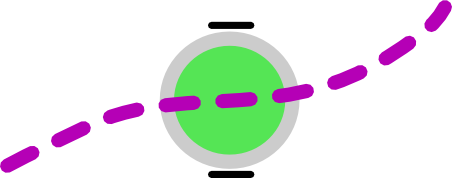
\includegraphics{gfx/activation.png}
		\caption{Gate activation}
	\label{fig:activation}
\end{figure}



\subsection{Menus}

The menus of this system are ring-shaped, with its options spread along the ring in the form or gates.
The menu's background ring is translucent so the main viewport remains visible and each background color
depends on the functionality it offers.
On the bottom-right area a curved label identifies the menu title.
The top-right area features additional gates for the dismissal of the menu, moving it around and
returning to the main menu if at a subsequent level (see Fig.\ref{fig:menu}).

\begin{figure}[ht]
	\centering
		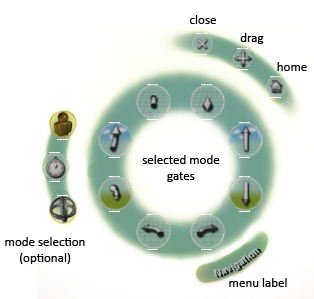
\includegraphics[scale=0.6]{gfx/menu.png}
	\caption{Menu and its areas}
	\label{fig:menu}
\end{figure}

A lot of effort has been put for menus to be usable. On cases where menus offered a large number of actions/options,
those were clustered into modes to keep a conveniently small number of visible options.
On such menus, a set of gates at the left side of the menu represent the available modes.
Selecting a different mode is a matter of activating the respective illustrative gate.

Additionally to splitting menu gates into modes, gates can be grouped by purpose.
On shape manipulation menus, gates which share similar functionality are clustered into
general purpose action gates. As an example: move, move neighbors and extrude operations are clustered,
as are bevel and beveled extrude. This solution favors Hick's Law as stated by Landauer and Nachbar \cite{MENU-TREES},
since it shows a smaller set of easily distinguishable options, with the user setting the exact action
he intends to reach from a smaller, filtered set of gates.



\subsection{Stroke Gestures}

To invoke the main menu the user needs to draw a closed stroke resembling a triangle (see Fig.\ref{fig:triangle}).
When such stroke is drawn one main menu instance appears centered on it.

\begin{figure}[ht]
	\centering
		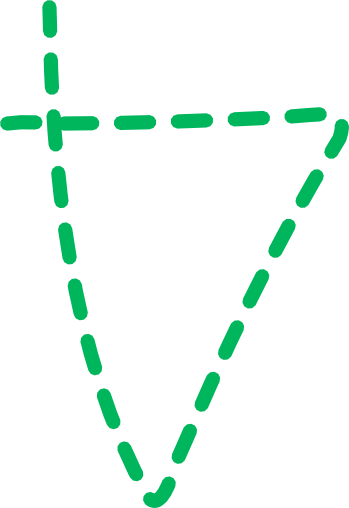
\includegraphics[scale=0.75]{gfx/triangle.png}
	\caption{Main menu stroke}
	\label{fig:triangle}
\end{figure}


Besides menus derived from the main menu tree, which is invoked as we've just seen by drawing a closed triangle stroke,
there are menus which focus on an existing shape on the 3D world.
These are called contextual menus and they can be invoked by selecting a desired shape's face or edge.
To select a face one has to draw a small stroke starting and ending inside the face.
To select an edge one has to draw a small stroke starting on one of the edge's neighboring faces and ending at the remaining one,
effectively crossing the edge to select it (see Fig.\ref{fig:face-edge-selection}).


\begin{figure}[ht]
	\centering
		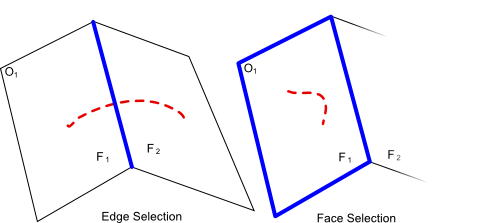
\includegraphics[scale=0.75]{gfx/face-edge-selection.png}
		\caption{Edge and Face selection}
	\label{fig:face-edge-selection}
\end{figure}


\subsection{Main Menu vs Contextual Menu}

Every action which generates new shapes is accessible from the main menu.
Actions which change existing contents are available from context menus for face and edge.
This segmentation rule was enforced so users know where to search when in need of an untried operation.


\section{Multimodal Input Interface}

Using laser input allows the usage of all system's functionalities.
Even so, an alternative arm-tracking and speech recognition command interface exists to enhance particular tasks.
The arms are tracked by attaching 2 reflective markers on each arm: one on each wrist and one close to each elbow.
Speech commands are obtained from a wireless headset attached to the user's ear (see Fig.\ref{fig:markers2}).


\begin{figure}[ht]
	\centering
		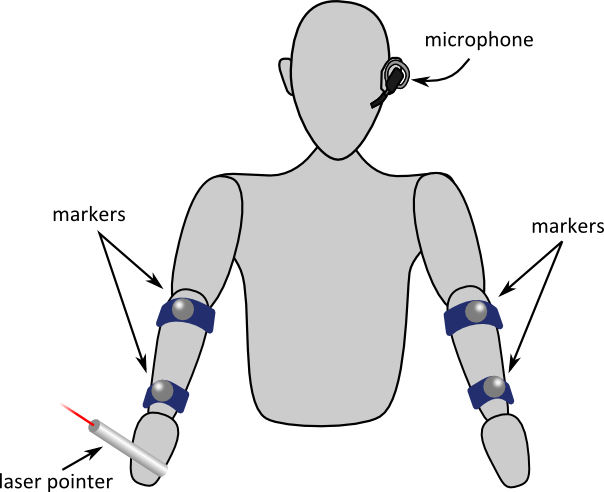
\includegraphics[scale=1.15]{gfx/markers2.png}
	\caption{user with reflective markers and wireless headset}
	\label{fig:markers2}
\end{figure}



\subsection{Arm Posing Flight Mode}
\label{FLIGHT-DESIGN-LABEL}

Given the available space in front of the large screen display and the existence of tracking hardware on the test lab,
an experimental mode was implemented, integrating the input extracted from tracking users arm movements and speech commands.
The idea is of offering a hands-on mode for flying.
The arm movements control both flight speed, rotation and altitude shift.
The voice commands are only required for controlling the application/inhibition of this mode.



\section{Content Creation Concepts}

\subsection{Apply-to-Scene Creation}
\label{design:apply-to-scene}

To create a new object on the scene one has to perform a stroke which activates the desired shape creation gate (cube for instance)
and continue the stroke onto the desired location where the shape is to rest. As soon as the gate is activated the shape appears
on top of the stroke and keeps following the stroke until it ends, offering a preview of the location where is would rest
if the stroke ended that particular moment (see Fig.\ref{fig:apply-to-scene}).
To figure out the actual location for the shape during the task the shape is iteratively collided against the
existing scene geometry so it stays in touch with the environment.

\begin{figure}[ht]
	\centering
		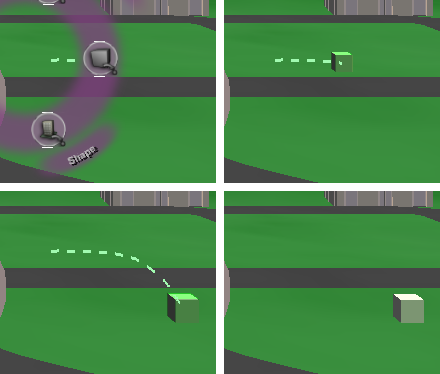
\includegraphics[scale=0.5]{gfx/apply-to-scene.png}
	\caption{Apply-to-scene procedure - creating a shape}
	\label{fig:apply-to-scene}
\end{figure}



\subsection{Instancing a Building}
\label{design:building}

To create a building one has to feed the system 3 parameters: building style, blueprint and height.
Due to the system decision for stroke-driven actions without global state, these 3 parameters are given with the
minimum strokes (2), as described next.
From a menu the list of supported building styles is presented to the user, each style a different gate.
Once activating the desired style the user starts an apply-to-scene process, moving a construction plane which must
be put where the blueprint is to be drawn.
The user draws a closed rectangle representing the blueprint and after closing it continues
the stroke upwards in order to define the building's height.
Once the stroke ends the building is generated according to the given parameters.
The construction plane has now carried out its purpose and therefore is terminated (see Fig.\ref{fig:building}).

\begin{figure}[ht]
	\centering
		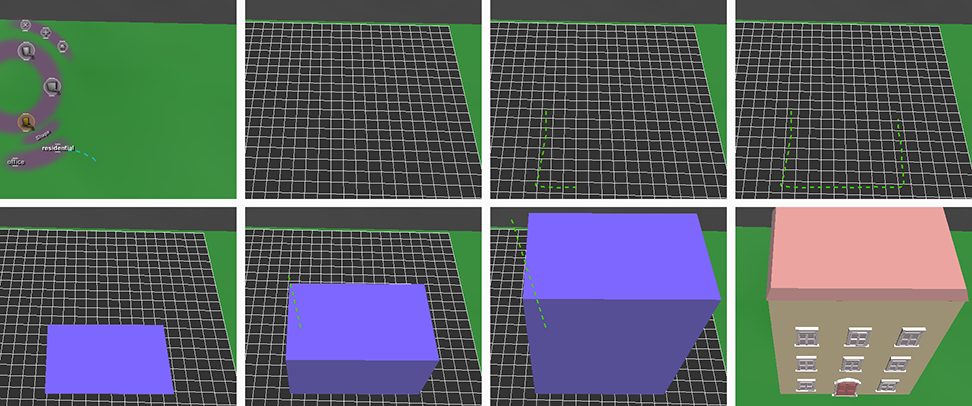
\includegraphics[scale=0.4]{gfx/building.png}
	\caption{Building creation procedure}
	\label{fig:building}
\end{figure}
